\section{Product and Evidence Architecture}

\subsection{Operating boundary}

FL-BSA is designed as a customer-hosted evidence appliance. A run accepts a tabular decision
snapshot, a declared outcome, protected-attribute mappings, and a statistical analysis plan. It
produces branch-specific synthetic tables, aggregate fairness and quality measures, certificates,
and provenance. This paper exercises the same evidence contract with a generated fixture; it does
not use borrower or customer data.

The v5.0.1 evidence selects the first-party evidence-native generator. The paper describes only the
selected release path and does not infer capabilities from unused backends. The runtime image is
bound by immutable digest
\IdentityText{\RuntimeImageDigestRaw}. The intake records the code commit, configuration hash,
canonical fixture hash, random seeds, workflow identity, and image digest required to locate the
run.

\begin{figure}[htbp]
  \centering
  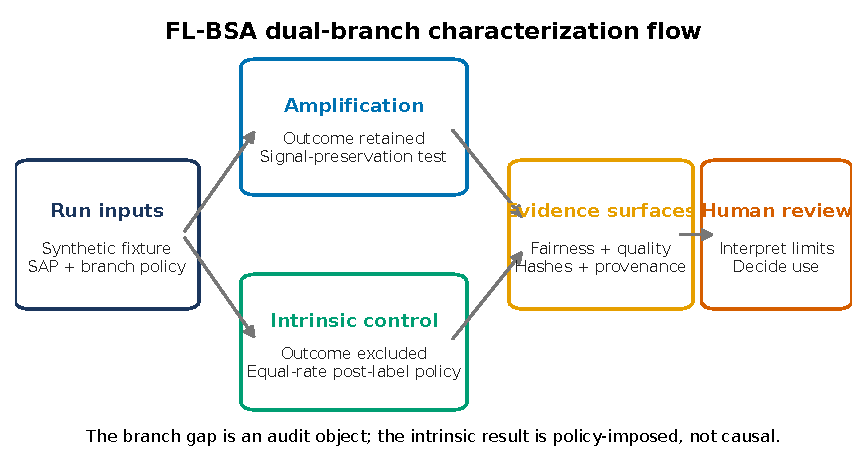
\includegraphics[
    alt={Flow diagram. A generated fixture and statistical policy split into an amplification branch that retains the outcome signal and an intrinsic control that excludes outcome aliases then applies an equal-rate post-label policy. Both feed fairness, quality and provenance evidence, followed by human review.},
    width=\linewidth
  ]{figures/characterization_architecture.pdf}
  \caption{The v5.0.1 dual-branch characterization flow. Human review remains outside the
  generator: evidence supports a decision; it does not make the governance or legal decision.}
  \label{fig:architecture}
\end{figure}

\subsection{Amplification branch}

The amplification branch is trained with the outcome surface present. Its purpose is to retain
observable decision associations strongly enough that a reviewer can test the downstream evidence
path. In this fixture, its gender AIR closely reproduces the historical value. That is evidence of
signal preservation for this run, not a claim that every dependency or subgroup distribution is
perfectly reproduced. Quality and utility are evaluated separately.

\subsection{Intrinsic parity-policy control}

Before intrinsic generation, the selected path excludes the declared outcome and known outcome
aliases. After generating the remaining columns, it applies a configured equal-rate labelling
policy across protected groups. Near-parity is therefore structurally expected. The branch is a
control for outcome-surface exclusion, post-label policy execution, and branch separation.

The intrinsic result cannot identify a causal mechanism. It does not simulate the same applicants
under an alternative lender policy, hold all confounders fixed, estimate potential outcomes, or
prove that the historical gap originated in decision labels. Throughout this paper it is called a
\emph{parity-policy control}, not a causal counterfactual.

\subsection{Evidence and publication chain}

\begin{figure}[htbp]
  \centering
  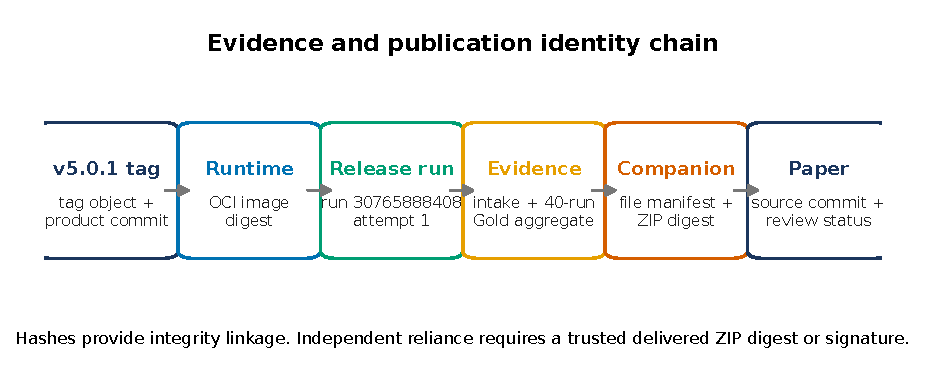
\includegraphics[
    alt={Evidence chain diagram from the annotated v5.0.1 tag and product commit, through an immutable runtime image and release workflow run, to the intake and forty-run Gold aggregate, the companion manifest and digest, and the source-bound candidate paper.},
    width=\linewidth
  ]{figures/characterization_evidence_chain.pdf}
  \caption{Identity chain used by this candidate. Hashes link exact bytes and predecessor records.
  Independent reliance still requires a trusted delivered digest or a verifiable external
  signature.}
  \label{fig:evidence-chain}
\end{figure}

The intake contains 21 certificate files. Three legacy-name files repeat canonical content under
the same content hash as branch-qualified files (their excluded signing timestamps differ), so the
content-hash graph has 18 distinct nodes, 17 distinct predecessor edges, and one root; all 20
non-root file entries resolve. The bundle also carries signature-shaped
metadata. Its public verification key is not in the whitepaper companion, and the intake intent
does not expect this intake pack to be cryptographically authoritative. Accordingly, this paper
claims \emph{integrity linkage}, not independent tamper proof. The companion ZIP digest on the
cover becomes an external check only when a reviewer receives that digest through a trusted
channel.
